\pagenumbering{arabic}
\chapter{Einleitung}
\label{cha:einleitung}
In der Softwareentwicklung hat in den letzten Jahren der Begriff des \textit{Reactive Programming} an Bedeutung gewonnen. Diese Erkenntnis zeigt auch die Abbildung \ref{pic:googletrend} der Google-Suchanfragen der letzten fünf Jahre zu diesem Thema. Noch deutlicher wird das Interesse, wenn man den \textit{Hype Cycle of Application Development 2016} von Gartner betrachtet \cite{cycle}. Hier ist Reactive Programming als klar aufstrebend in der Skala der neuen Technologien gelistet, welche sich jedoch noch in der Praxis etablieren müssen. Eine Anwendung die auf Ereignis reagiert ist jedoch nichts neues und kann mit den bereit vorhanden Programmierparadigmen realisiert werden. Es stellt sich die Frage wieso sich nun ein neues Paradigma entwickelt hat und was die besonderen Eigenschaften des Reactive Programming sind. Wenn wie angesprochen eine Reaktion auf auftretende Ereignisse von der Anwendung möglich ist, bezeichnet man diese als interaktiv. Die Häufigkeit für das Auftreten von Ereignissen wird durch den Benutzer oder ein weiteres Programm kontrolliert. Tritt ein Ereignis auf, führt das Programm den damit verbunden Codeabschnitt aus wie zum Beispiel eine Berechnung. Während dieser Vorgang läuft wartet das Programm und liefert nach Abschluss der Aufgabe ein Resultat. Der eigentliche Programmfluss kann anschließend fortgesetzt werden. Dieses Verhalten wird häufig durch die Verwendung des Observer-Pattern erreicht. Betrachtet man dagegen ein reaktives Verhalten kommen zu der vorhandenen Interaktivität weitere Aspekte hinzu. Es soll ermöglicht werden die Ereignisse asynchron zu verarbeiten. Ebenso soll die Anwendung während dieser Verarbeitung nicht blockieren, und somit zu jeder Zeit antwortbereit bleiben. Ziel von Reactive Programming ist es diese Eigenschaften in einem neuem Programmierparadigma zu vereinen.
\begin{figure}[hbt]
	\centering
	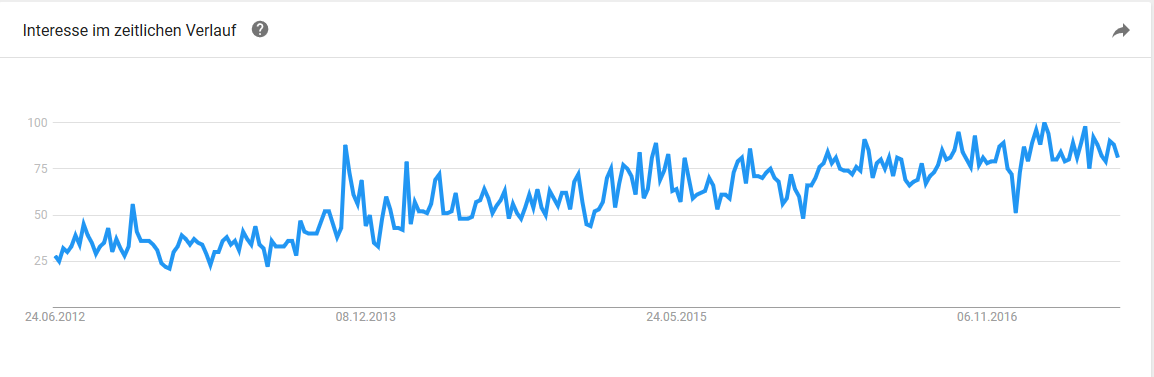
\includegraphics[width=1\textwidth]{Abb/rptrend}
	\caption{Verhältnis von Google Suchanfragen zum Thema Reactive Programming seit 2012.}
	\label{pic:googletrend}
\end{figure}
\section{Zielsetzung}
Diese Arbeit hat zum Ziel einen Überblick über dieses neue Paradigma zu geben. Es soll geklärt werden welche Bestandteile notwendig sind um eine Applikation reaktiv zu entwickeln. Diese Komponenten sollen separat beschrieben werden, aber auch eine Einordnung in den Kontext von kompletten Systemen soll vorgenommen werden. Zur Veranschaulichung soll eine Referenzbibliothek, welche diesen Prinzipien folgt, im Details beschrieben werden und eine beispielhafte Anwendung mit Verwendung dieser Bibliothek soll den Einblick in die Grundlagen des Themas Reactive Programming abschließen.
\section{Aufbau der Arbeit}
Um diese Ziele zu erreichen kann die Arbeit prinzipiell in zwei Bereiche unterteilt werden. Der erste Teil umfasst die Theorie zum Thema Reactive Programming. Es wird geschildert was \textit{reactive} im Kontext der Softwareentwicklung bedeutet. Weiterhin findet eine Unterscheidung zwischen Reactive Systems und Reactive Programming statt. Anschließend an die Differenzierung wird geklärt welche Bausteine notwendig sind, um ein Verhalten wie es Reactive Programming vorsieht zu entwickeln. Der darauffolgende praktischere Teil beschreibt eine konkrete Implementierung dieser Bausteine in der Bibliothek RxJava2. Das Verhalten dieser Bibliothek mit Themen wie Asynchronität oder Nebenläufigkeit und Beispielimplementierungen der Basisklassen werden behandelt. Als Beispielapplikation wird ein Systemmonitor mit Verwendung dieser Bibliothek implementiert und die verwendeten Bestandteile genauer beschrieben. Abschließend wird eine Einschätzung für relevante Einsatzmöglichkeiten durchgeführt.
